\newpage
\hypertarget{TGGSchema}{}
\section{Creating your TGG schema}
\genHeader

Now that the necessary source and target metamodels are in the same workspace, there are several different ways to begin specifying a TGG. We're going to start
with modeling the correspondence component of the triple language. This correspondence, or \emph{link metamodel},\define{Link \\ Metamodel} specifies
\emph{correspondence types},\define{Correspondence Types} which will be used to connect specific elements of the source and target metamodels. These
correspondence elements can also be thought of as \emph{traceability links}.

While the link metamodel is technically a standard metamodel, eMoflon uses a slightly different naming convention and concrete syntax to represent it. The
overall\define{TGG Schema} metamodel triple consisting of the relevant parts of the source, link, and target metamodels is called a \emph{TGG schema}.

A TGG schema can be viewed as the (metamodel) triple to which all \emph{new} triples must conform. In less technical lingo, it gives an abstract view on the
relationships (correspondence) between two metamodels or domains. A domain expert should be able to understand why certain connected elements are related,
irrespective of how the relationship is actually established by TGG rules, just by looking at the TGG schema. 

In our example schema, we will create a link between our source \texttt{Box} and target \texttt{Dictionary} to express that these two container elements are
related.

\jumpDual{schema vis}{schema tex}

\newpage
\hypertarget{schema vis}{}
\subsection{Visual Schema}
\visHeader

\begin{itemize}

\item[$\blacktriangleright$] Open \texttt{LearningBox2Dictionary.eap} in EA, and add a new package to \texttt{MyWorkingSet} (your model root) with
\texttt{Learning\-Box\-To\-Dictionary\-Integration} as its name (Fig.~\ref{fig:intgPackage}). 

\vspace{0.5cm}

\begin{figure}[htbp]
\begin{center}
  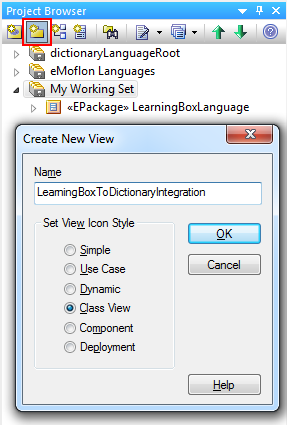
\includegraphics[width=0.4\textwidth]{ea_integrationPackage}
  \caption{Create a new package}  
  \label{fig:intgPackage}
\end{center}
\end{figure}


\item[$\blacktriangleright$] Create a diagram in the new package, selecting \texttt{TGGSchema} as diagram type (Fig.~\ref{fig:tgg_diagram_type}). The diagram
type indicates to EA that the new package is a TGG Project.

\vspace{0.5cm}

\begin{figure}[htbp]
\begin{center}
  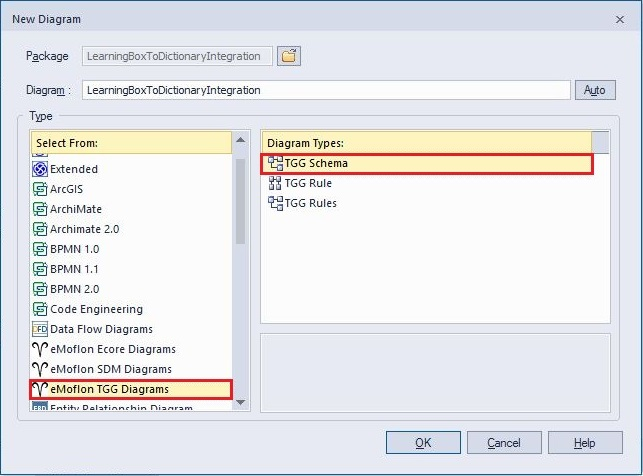
\includegraphics[width=0.9\textwidth]{ea_newTGGSchema}
  \caption{Choose \texttt{TGGSchema} as your diagram type}  
  \label{fig:tgg_diagram_type}
\end{center}
\end{figure}

\item[$\blacktriangleright$] After choosing \texttt{TGGSchema} as diagram type, a new dialogue should pop up asking you for the source and target projects of your TGG project. 
Choose \texttt{Learning\-Box\-Language} as source and \texttt{Dictionary\-Language} as target project and affirm with \texttt{OK} (Fig.~\ref{fig:select_source_target}).

\vspace{0.5cm}

\begin{figure}[htbp]
\begin{center}
  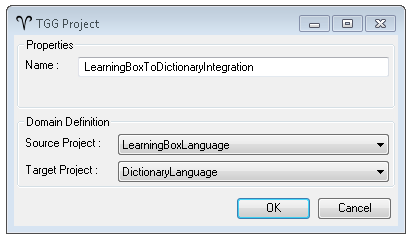
\includegraphics[width=0.55\textwidth]{ea_TGGSourceTarget}
  \caption{Select source and target projects for the TGG project}  
  \label{fig:select_source_target}
\end{center}
\end{figure}

\item[$\blacktriangleright$] The structure of your TGG project should now resemble Fig.~\ref{fig:new_tgg_project}. Please note that a subpackage \texttt{Rules}
and an underlying diagram with the same name are also generated.

\begin{figure}[htbp]
\begin{center}
  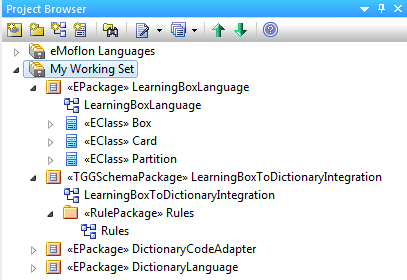
\includegraphics[width=0.5\textwidth]{ea_browserPostDiagram}
  \caption{Initial structure of a new TGG project}  
  \label{fig:new_tgg_project}
\end{center}
\end{figure}
\end{itemize}
\clearpage

Now it's time to insert classes from our source and target projects into our TGG project and declare our first \emph{correspondence type} between them.
The classes \texttt{Box} and \texttt{Dictionary} are to be related to each other.

\begin{itemize}
\item[$\blacktriangleright$] Hold \texttt{ctrl}, then drag-and-drop the \texttt{Box} class from \texttt{Learning\-Box\-Language} into the newly created TGG
schema diagram, which should have automatically opened in the editor when you made it. Ensure that the class is pasted \texttt{as a simple link} into the
diagram (Fig.)

\begin{figure}[htbp]
\begin{center}
  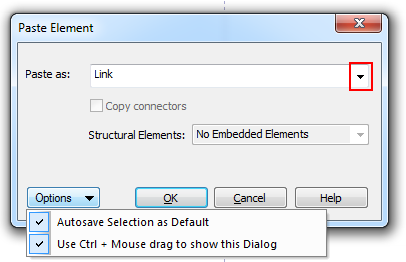
\includegraphics[width=0.6\textwidth]{ea_TGGDragDrop}
  \caption{Copying an element as a simple link} 
  \label{fig:TGGdragDrop}
\end{center}
\end{figure}

\item[$\blacktriangleright$] If you selected the \texttt{Autosave Selection as default} option during the previous drag and drop, you no longer need to hold
\texttt{ctrl} to bring the \texttt{Dictionary} class from \texttt{Dictionary\-Language} into the TGG schema.
\end{itemize}

With a class from both source and target projects, we can now create a correspondence type between them.

\begin{itemize}
\item[$\blacktriangleright$] Quick-link from \texttt{Box} to \texttt{Dictionary} and select \texttt{Create TGG Corres\-pon\-dence Type} as depicted in
Fig.~\ref{fig:create_correspondence}.
\end{itemize}

\begin{figure}[htbp]
\begin{center}
  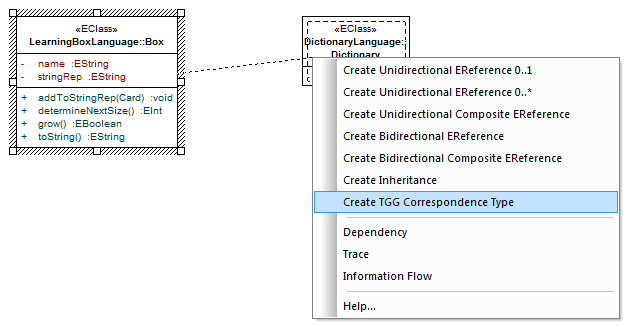
\includegraphics[width=\textwidth]{ea_TGGCorrespType}
  \caption{Creating a TGG correspondence type} 
  \label{fig:create_correspondence}
\end{center}
\end{figure}

A hexagon-shaped correspondence type named \texttt{BoxToDiction\-ary}, and references to each source and target element should have been generated.
You can rename the type as you wish, but please leave the references as they are (multiplicity and naming conventions are satisfied automatically).

To finish our TGG schema, declare a second correspondence type in the same file between \texttt{Card} and \texttt{Entry}. You'll notice that the
reference between \texttt{Dictionary} and \texttt{Entry} was automatically created! Your completed TGG Schema should resemble
Fig.~\ref{fig:complete_tgg_schema}.

\begin{figure}[htbp]
\begin{center}
  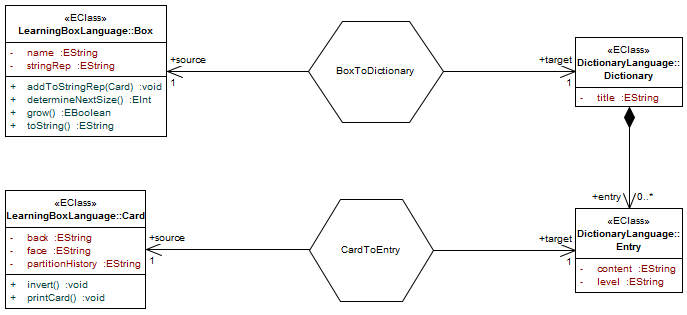
\includegraphics[width=\textwidth]{ea_completeTGGSchema}
  \caption{Complete TGG schema for our example}
  \label{fig:complete_tgg_schema}
\end{center}
\end{figure}



\newpage
\hypertarget{schema tex}{}
\subsection{Textual TGG Schema}
\texHeader

\begin{itemize}

\item[$\blacktriangleright$] Within the learning box metamodel folder, right-click on \texttt{MyWorkingSet}, and navigate to ``New / TGG''
(Fig.~\ref{eclipse:contextTGG}).

\vspace{0.5cm}

\begin{figure}[htbp]
\begin{center}
  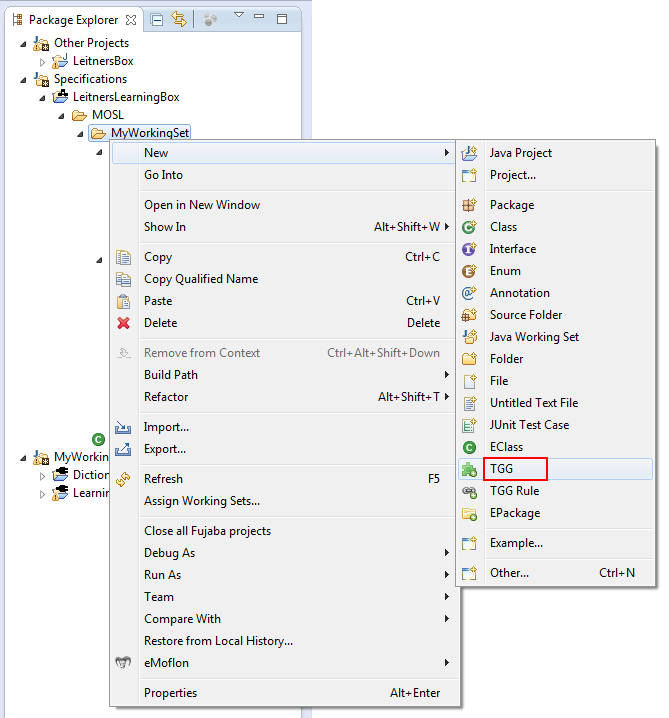
\includegraphics[width=0.8\textwidth]{eclipse_contextNewTGG}
  \caption{Creating a new TGG schema}
  \label{eclipse:contextTGG}
\end{center}
\end{figure}

\item[$\blacktriangleright$] Name the TGG \texttt{LearningBoxToDictionaryIntegration}, setting the source as \texttt{LearningBoxLanguage}, and target as
\texttt{DictionaryLanguage} (Fig.~\ref{eclipse:newTGG}).

\vspace{0.5cm}

\item[$\blacktriangleright$] A new TGG \texttt{schema} file should now be active in the editor! This is the \emph{TGG Schema} which declares each
\emph{correspondence type} as an \texttt{integration class}. Press \texttt{ctrl + space bar} and use the auto completion to generate a new integration class.

\newpage

\begin{figure}[htbp]
\begin{center}
  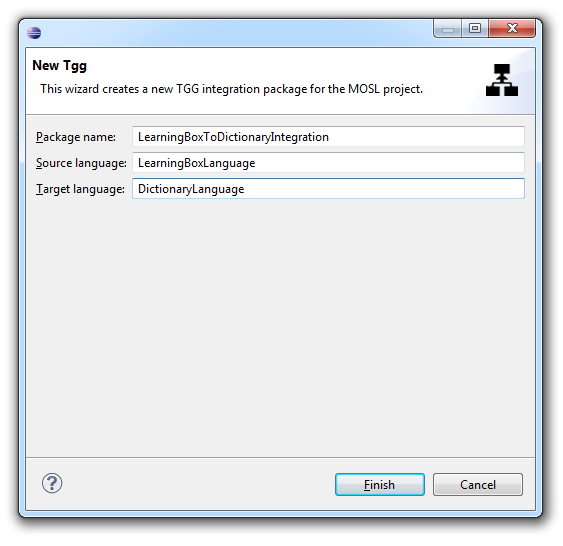
\includegraphics[width=0.8\textwidth]{eclipse_newTGG}
  \caption{Setting your \texttt{source} and \texttt{target} metamodels}
  \label{eclipse:newTGG}
\end{center}
\end{figure}

\item[$\blacktriangleright$] Note that when using a template, you can press \texttt{tab} to cycle through each element. Name the class
\texttt{BoxToDictionary}, and list the source as \texttt{Box} and target as \texttt{Dictionary} (Fig.~\ref{eclipse:firstCorrType}). 

\begin{figure}[htbp]
\begin{center}
  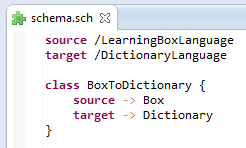
\includegraphics[width=0.4\textwidth]{eclipse_schemaFirstClass}
  \caption{Creating a correspondence type}
  \label{eclipse:firstCorrType}
\end{center}
\end{figure}

\item[$\blacktriangleright$] Believe it or not, that's all you need for your first correspondence type! Your schema is now complete with connections to your
\texttt{source} and \texttt{target} metamodels via a \emph{link} metamodel. To see the equivalent structure in the visual syntax, check out
Fig.~\ref{ea:firstCorrType} from the previous section.

\end{itemize}

